% Options for packages loaded elsewhere
\PassOptionsToPackage{unicode}{hyperref}
\PassOptionsToPackage{hyphens}{url}
\PassOptionsToPackage{dvipsnames,svgnames,x11names}{xcolor}
%
\documentclass[
  letterpaper,
  DIV=11]{scrreprt}

\usepackage{amsmath,amssymb}
\usepackage{lmodern}
\usepackage{iftex}
\ifPDFTeX
  \usepackage[T1]{fontenc}
  \usepackage[utf8]{inputenc}
  \usepackage{textcomp} % provide euro and other symbols
\else % if luatex or xetex
  \usepackage{unicode-math}
  \defaultfontfeatures{Scale=MatchLowercase}
  \defaultfontfeatures[\rmfamily]{Ligatures=TeX,Scale=1}
\fi
% Use upquote if available, for straight quotes in verbatim environments
\IfFileExists{upquote.sty}{\usepackage{upquote}}{}
\IfFileExists{microtype.sty}{% use microtype if available
  \usepackage[]{microtype}
  \UseMicrotypeSet[protrusion]{basicmath} % disable protrusion for tt fonts
}{}
\makeatletter
\@ifundefined{KOMAClassName}{% if non-KOMA class
  \IfFileExists{parskip.sty}{%
    \usepackage{parskip}
  }{% else
    \setlength{\parindent}{0pt}
    \setlength{\parskip}{6pt plus 2pt minus 1pt}}
}{% if KOMA class
  \KOMAoptions{parskip=half}}
\makeatother
\usepackage{xcolor}
\setlength{\emergencystretch}{3em} % prevent overfull lines
\setcounter{secnumdepth}{5}
% Make \paragraph and \subparagraph free-standing
\ifx\paragraph\undefined\else
  \let\oldparagraph\paragraph
  \renewcommand{\paragraph}[1]{\oldparagraph{#1}\mbox{}}
\fi
\ifx\subparagraph\undefined\else
  \let\oldsubparagraph\subparagraph
  \renewcommand{\subparagraph}[1]{\oldsubparagraph{#1}\mbox{}}
\fi


\providecommand{\tightlist}{%
  \setlength{\itemsep}{0pt}\setlength{\parskip}{0pt}}\usepackage{longtable,booktabs,array}
\usepackage{calc} % for calculating minipage widths
% Correct order of tables after \paragraph or \subparagraph
\usepackage{etoolbox}
\makeatletter
\patchcmd\longtable{\par}{\if@noskipsec\mbox{}\fi\par}{}{}
\makeatother
% Allow footnotes in longtable head/foot
\IfFileExists{footnotehyper.sty}{\usepackage{footnotehyper}}{\usepackage{footnote}}
\makesavenoteenv{longtable}
\usepackage{graphicx}
\makeatletter
\def\maxwidth{\ifdim\Gin@nat@width>\linewidth\linewidth\else\Gin@nat@width\fi}
\def\maxheight{\ifdim\Gin@nat@height>\textheight\textheight\else\Gin@nat@height\fi}
\makeatother
% Scale images if necessary, so that they will not overflow the page
% margins by default, and it is still possible to overwrite the defaults
% using explicit options in \includegraphics[width, height, ...]{}
\setkeys{Gin}{width=\maxwidth,height=\maxheight,keepaspectratio}
% Set default figure placement to htbp
\makeatletter
\def\fps@figure{htbp}
\makeatother
\newlength{\cslhangindent}
\setlength{\cslhangindent}{1.5em}
\newlength{\csllabelwidth}
\setlength{\csllabelwidth}{3em}
\newlength{\cslentryspacingunit} % times entry-spacing
\setlength{\cslentryspacingunit}{\parskip}
\newenvironment{CSLReferences}[2] % #1 hanging-ident, #2 entry spacing
 {% don't indent paragraphs
  \setlength{\parindent}{0pt}
  % turn on hanging indent if param 1 is 1
  \ifodd #1
  \let\oldpar\par
  \def\par{\hangindent=\cslhangindent\oldpar}
  \fi
  % set entry spacing
  \setlength{\parskip}{#2\cslentryspacingunit}
 }%
 {}
\usepackage{calc}
\newcommand{\CSLBlock}[1]{#1\hfill\break}
\newcommand{\CSLLeftMargin}[1]{\parbox[t]{\csllabelwidth}{#1}}
\newcommand{\CSLRightInline}[1]{\parbox[t]{\linewidth - \csllabelwidth}{#1}\break}
\newcommand{\CSLIndent}[1]{\hspace{\cslhangindent}#1}

\KOMAoption{captions}{tableheading}
\makeatletter
\makeatother
\makeatletter
\@ifpackageloaded{bookmark}{}{\usepackage{bookmark}}
\makeatother
\makeatletter
\@ifpackageloaded{caption}{}{\usepackage{caption}}
\AtBeginDocument{%
\ifdefined\contentsname
  \renewcommand*\contentsname{Inhaltsverzeichnis}
\else
  \newcommand\contentsname{Inhaltsverzeichnis}
\fi
\ifdefined\listfigurename
  \renewcommand*\listfigurename{Abbildungsverzeichnis}
\else
  \newcommand\listfigurename{Abbildungsverzeichnis}
\fi
\ifdefined\listtablename
  \renewcommand*\listtablename{Tabellenverzeichnis}
\else
  \newcommand\listtablename{Tabellenverzeichnis}
\fi
\ifdefined\figurename
  \renewcommand*\figurename{Abbildung}
\else
  \newcommand\figurename{Abbildung}
\fi
\ifdefined\tablename
  \renewcommand*\tablename{Tabelle}
\else
  \newcommand\tablename{Tabelle}
\fi
}
\@ifpackageloaded{float}{}{\usepackage{float}}
\floatstyle{ruled}
\@ifundefined{c@chapter}{\newfloat{codelisting}{h}{lop}}{\newfloat{codelisting}{h}{lop}[chapter]}
\floatname{codelisting}{Listing}
\newcommand*\listoflistings{\listof{codelisting}{Listingverzeichnis}}
\makeatother
\makeatletter
\@ifpackageloaded{caption}{}{\usepackage{caption}}
\@ifpackageloaded{subcaption}{}{\usepackage{subcaption}}
\makeatother
\makeatletter
\@ifpackageloaded{tcolorbox}{}{\usepackage[many]{tcolorbox}}
\makeatother
\makeatletter
\@ifundefined{shadecolor}{\definecolor{shadecolor}{rgb}{.97, .97, .97}}
\makeatother
\makeatletter
\makeatother
\ifLuaTeX
\usepackage[bidi=basic]{babel}
\else
\usepackage[bidi=default]{babel}
\fi
\babelprovide[main,import]{ngerman}
% get rid of language-specific shorthands (see #6817):
\let\LanguageShortHands\languageshorthands
\def\languageshorthands#1{}
\ifLuaTeX
  \usepackage{selnolig}  % disable illegal ligatures
\fi
\IfFileExists{bookmark.sty}{\usepackage{bookmark}}{\usepackage{hyperref}}
\IfFileExists{xurl.sty}{\usepackage{xurl}}{} % add URL line breaks if available
\urlstyle{same} % disable monospaced font for URLs
\hypersetup{
  pdftitle={Business Analytics \& Coding},
  pdflang={de},
  colorlinks=true,
  linkcolor={blue},
  filecolor={Maroon},
  citecolor={Blue},
  urlcolor={Blue},
  pdfcreator={LaTeX via pandoc}}

\title{Business Analytics \& Coding}
\author{}
\date{}

\begin{document}
\maketitle
\ifdefined\Shaded\renewenvironment{Shaded}{\begin{tcolorbox}[interior hidden, enhanced, frame hidden, breakable, boxrule=0pt, borderline west={3pt}{0pt}{shadecolor}, sharp corners]}{\end{tcolorbox}}\fi

\renewcommand*\contentsname{Inhaltsverzeichnis}
{
\hypersetup{linkcolor=}
\setcounter{tocdepth}{2}
\tableofcontents
}
\bookmarksetup{startatroot}

\hypertarget{vorwort}{%
\chapter*{VORWORT}\label{vorwort}}
\addcontentsline{toc}{chapter}{VORWORT}

\markboth{VORWORT}{VORWORT}

Bei diesem Skript handelt es sich um Selbstlernmaterial zum Thema
\texttt{Datenanalyse}. Noch konkreter beschäftigt sich dieses Skript mit
\texttt{Business\ Analytics}. Das Skript wurde neu konzipiert und
richtet sich explizit an
\texttt{Studierende\ der\ Betriebswirtschaftlehre}. Aktuell ``atmet''
das Dokument noch, d.h. Aktualisierungen und Ergänzungen sind
wahrscheinlich. Auch werden perspektivisch fortgeschrittenere
Themenblöcke zum Bereich der \texttt{Predictive\ Analytics} ergänzt
werden.

Das Skript ist explizit mit dem Ziel verfasst, als Selbstlernmaterial
verwendet zu werden. Zumindest ist dies beim Verfassen des Skripts immer
meine ausdrückliche Intention gewesen. Alle Code-Beispiele können via
Knopfdruck selbst ausprobiert und adaptiert werden. Das Dokument ist
somit zu Teilen interaktiv und sollte deshalb auch nicht nur passiv
konsumiert werden.

Ob mein Vorhaben tatsächlich gelungen ist, können schlussendlich nur Sie
beurteilen. Sollten Sie also Fragen oder Anmerkungen bzw. technische
Probleme haben oder - und dies bleibt leider nie aus - Fehler entdecken,
dann bin ich dankbar für Ihr Feedback. Sprechen Sie mich entweder in den
Veranstaltungen zum Modul direkt an oder schreiben mir eine Email
(\texttt{felix.zeidler{[}at{]}fh-bielefeld.de}). Auch wenn es mir
vermutlich nicht immer gelingen wird, Ihnen direkt zu antworten, bin ich
dankbar für jede Art von Rückmeldung.

Viel Spaß beim Lesen und Ausprobieren!

\hypertarget{header-2}{%
\section*{Header 2}\label{header-2}}
\addcontentsline{toc}{section}{Header 2}

\markright{Header 2}

Hier steht ein Text

\hypertarget{header-3}{%
\subsection*{Header 3}\label{header-3}}
\addcontentsline{toc}{subsection}{Header 3}

Bei diesem Skript handelt es sich um Selbstlernmaterial zum Thema
\texttt{Datenanalyse}. Noch konkreter beschäftigt sich dieses Skript mit
\texttt{Business\ Analytics}. Das Skript wurde neu konzipiert und
richtet sich explizit an
\texttt{Studierende\ der\ Betriebswirtschaftlehre}. Aktuell ``atmet''
das Dokument noch, d.h. Aktualisierungen und Ergänzungen sind
wahrscheinlich. Auch werden perspektivisch fortgeschrittenere
Themenblöcke zum Bereich der \texttt{Predictive\ Analytics} ergänzt
werden.

Das Skript ist explizit mit dem Ziel verfasst, als Selbstlernmaterial
verwendet zu werden. Zumindest ist dies beim Verfassen des Skripts immer
meine ausdrückliche Intention gewesen. Alle Code-Beispiele können via
Knopfdruck selbst ausprobiert und adaptiert werden. Das Dokument ist
somit zu Teilen interaktiv und sollte deshalb auch nicht nur passiv
konsumiert werden.

Ob mein Vorhaben tatsächlich gelungen ist, können schlussendlich nur Sie
beurteilen. Sollten Sie also Fragen oder Anmerkungen bzw. technische
Probleme haben oder - und dies bleibt leider nie aus - Fehler entdecken,
dann bin ich dankbar für Ihr Feedback. Sprechen Sie mich entweder in den
Veranstaltungen zum Modul direkt an oder schreiben mir eine Email
(\texttt{felix.zeidler{[}at{]}fh-bielefeld.de}). Auch wenn es mir
vermutlich nicht immer gelingen wird, Ihnen direkt zu antworten, bin ich
dankbar für jede Art von Rückmeldung.

Viel Spaß beim Lesen und Ausprobieren!

\hypertarget{header-2-2}{%
\section*{Header 2 2}\label{header-2-2}}
\addcontentsline{toc}{section}{Header 2 2}

\markright{Header 2 2}

\part{EINLEITUNG}

This is a book created from markdown and executable code.

See Knuth (1984) for additional discussion of literate programming.

\hypertarget{einfuxfchrung-business-analytics}{%
\chapter{Einführung Business
Analytics}\label{einfuxfchrung-business-analytics}}

\hypertarget{was-ist-business-analytics}{%
\section{Was ist Business Analytics?}\label{was-ist-business-analytics}}

Bevor wir uns mit \textbf{Business Analytics} inhaltlich weitergehend
beschäftigen, müssen wir zunächst definieren, was der Begriff konkret
meint. Im Kontext dieser Veranstaltung definieren wir Business Analytics
als

\begin{quote}
``Ein Prozess zur Analyse von Daten mit dem Ziel unternehmerische
Entscheidungen zu unterstützen und zu verbessern.''
\end{quote}

Der Begriff Business Analytics wird in der Literatur unterschiedlich
definiert.\footnote{siehe z.B. Seiter (2019) oder {[}\textbf{TODO}{]}}
Für manche Autoren umfasst er alle Formen der Analyse von
Unternehmensdaten, während andere eine engere Definition bevorzugen, die
sich auf die Verwendung von maschinellen Lernverfahren und anderen
fortgeschrittenen Analysemethoden konzentriert. Trotz dieser
Unterschiede in der Definition haben alle Ansätze zu Business Analytics
eines gemeinsam: Sie zielen darauf ab, \textbf{durch die Analyse von
Daten unternehmerische Entscheidungen zu unterstützen und zu
verbessern}. Business Analytics ist daher als wichtige Disziplin zu
betrachten, die Unternehmen dabei hilft, ihre Leistung zu steigern und
ihre Entscheidungen datengestützt zu treffen.

Der Fokus von Business Analytics auf unternehmerische Entscheidungen
macht es zu einem wichtigen Thema für kaufmännische Funktionen innerhalb
von Unternehmen. Denn gerade in diesen Bereichen werden häufig
Entscheidungen getroffen, die den Erfolg und die Leistung des
Unternehmens beeinflussen. Business Analytics kann dabei helfen,
wichtige Daten und Insights zu sammeln und zu analysieren, um die
Entscheidungsfindung zu unterstützen und die Effektivität von Strategien
und Maßnahmen zu verbessern. Daher ist es wichtig, dass Führungskräfte
und Mitarbeiter in kaufmännischen Funktionen sich mit den Konzepten und
Methoden von Business Analytics auseinandersetzen und lernen, wie sie
diese in ihrer täglichen Arbeit anwenden können.

In der untenstehenden Tabelle~\ref{tbl-ba} sind ein paar beispielhafte
Anwendungsfälle dargestellt, die verdeutlichen, wie breit die Anwendung
von Business Analytics ist:

\hypertarget{tbl-ba}{}
\begin{longtable}[]{@{}
  >{\raggedright\arraybackslash}p{(\columnwidth - 4\tabcolsep) * \real{0.1143}}
  >{\raggedright\arraybackslash}p{(\columnwidth - 4\tabcolsep) * \real{0.2286}}
  >{\raggedright\arraybackslash}p{(\columnwidth - 4\tabcolsep) * \real{0.6571}}@{}}
\caption{\label{tbl-ba}Beispiele für Business Analytics}\tabularnewline
\toprule()
\begin{minipage}[b]{\linewidth}\raggedright
Funktion
\end{minipage} & \begin{minipage}[b]{\linewidth}\raggedright
Anwendungsfall
\end{minipage} & \begin{minipage}[b]{\linewidth}\raggedright
Beispiel
\end{minipage} \\
\midrule()
\endfirsthead
\toprule()
\begin{minipage}[b]{\linewidth}\raggedright
Funktion
\end{minipage} & \begin{minipage}[b]{\linewidth}\raggedright
Anwendungsfall
\end{minipage} & \begin{minipage}[b]{\linewidth}\raggedright
Beispiel
\end{minipage} \\
\midrule()
\endhead
Marketing & Wirksamkeit von Marketingkampagnen analysieren und
optimieren & ein Unternehmen könnte die Conversion-Rate von Landing
Pages oder die Klickrate von Email-Kampagnen analysieren, um zu
verstehen, welche Maßnahmen am effektivsten sind \\
Finanzen & finanzielle Leistung analysieren und optimieren & ein
Unternehmen könnte die Rentabilität von einzelnen Produkten oder
Geschäftsbereichen analysieren, um Ressourcen gezielt einzusetzen und
die Profitabilität zu erhöhen \\
Personal & Mitarbeiterleistung analysieren und verbessern & ein
Unternehmen könnte Daten zu Mitarbeiterfeedback, Absentismus und
Fluktuation analysieren, um die Mitarbeiterzufriedenheit und
-fluktuation zu erhöhen \\
Logistik & Leistung der Lieferkette analysieren und optimieren & ein
Unternehmen könnte Daten zu Lieferzeiten, Bestandsniveaus und
Transportkosten analysieren, um die Effizienz der Lieferkette zu erhöhen
und Lieferprobleme zu minimieren \\
\bottomrule()
\end{longtable}

Es wird außerdem deutlich, dass sich abhängig vom jeweiligen
Anwendungsfall auch die verwendeten Daten und Analysetechniken
unterscheiden können.

\hypertarget{vorteile-durch-business-analytics}{%
\section{Vorteile durch Business
Analytics?}\label{vorteile-durch-business-analytics}}

Ausgehend von der o.g. Definition kann die Datenanalyse auf sowohl
strategischer, als auch auf operativer Ebene vorteilhaft sein.

Auf operativer Ebene kann Der Einsatz von Business Analytics vorteilhaft
sein, da er es Unternehmen ermöglicht, Daten zu sammeln und zu
analysieren, um z.B. ihre Prozesse zu optimieren und/oder Kosten zu
senken. Auf Basis dieser Verbesserungen kann man sich vom Wettbewerb
unterscheiden und absetzen. Der Einsatz von Business Analytics kann auf
strategischer Ebene vorteilhaft sein, da er es Unternehmen ermöglicht,
Trends zu erkennen und auf sie zu reagieren, um sich einen
Wettbewerbsvorteil zu verschaffen. Die Analyse von Daten kann
Unternehmen dabei helfen, tiefgreifende Einblicke in die Märkte und
Kundenbedürfnisse zu gewinnen und diese Informationen zu nutzen, um ihre
Strategien anzupassen und sich von ihren Wettbewerbern abzuheben. Der
Einsatz von Business Analytics kann somit dazu beitragen, dass
Unternehmen ihre Wettbewerbsposition verbessern und ihre Leistung
steigern.

So ist es nicht verwunderlich, dass es auch Belege dafür gibt, dass
Unternehmen durch den Einsatz von Business Analytics erfolgreicher sind.
So zeigen z.B. Shanks u.~a. (2010) theoretisch auf, dass Business
Analytics einen Einfluss auf die Strategie und die Performance von
Unternehmen hat. Die vergleichende empirische Analyse von Popovič u.~a.
(2018) betont hingegen, dass Unternehmen, die hohen ``Business
Analytics''-Fähigkeiten haben, in der Lage sind bessere Entscheidungen
zu treffen und so einen höheren Unternehmenswert generieren. In einer
weiteren empirischen Analyse zeigen Almazmomi, Ilmudeen, und Qaffas
(2021), dass der erhöhte Einsatz von Business Analytics einen
Wettbewerbsvorteil darstellt.

\hypertarget{drei-arten-der-datenanalyse}{%
\section{Drei Arten der
Datenanalyse}\label{drei-arten-der-datenanalyse}}

Das Feld von Business Analytics ist sehr weit. Es macht deshalb Sinn,
das breite Themengebiet zu unterteilen. Wir werden im Rahmen dieses
Kurses Business Analytics in die folgenden drei Analyse-Kategorien
unterteilen:

\begin{enumerate}
\def\labelenumi{\arabic{enumi}.}
\item
  deskriptive Analyse
\item
  diagnostische Analyse
\item
  prädiktive Analyse
\end{enumerate}

Ich gebe zu: die Unterteilung ist ein Stück weit beliebig und auch nicht
MECE (mutual exclusive, collectively exhaustive). Ich halte Sie aus
didaktischen Gründen dennoch geeignet sich dem breiten Themengebiet
Business Analytics Schritt für Schritt zu nähern.\footnote{Für eine
  ausführlichere Diskussion der unterschiedlichen Arten von Business
  Analytics siehe z.B. Gluchowski (2016).}

Die \textbf{deskriptive Analytik} ist die Art von Business Analytics,
die sich auf die Vergangenheit konzentriert. Sie zielt darauf ab, ein
besseres Verständnis dafür zu entwickeln, was in der Vergangenheit
passiert ist, indem sie Daten sammelt und analysiert. Zum Beispiel
könnte ein Unternehmen die Verkaufszahlen der vergangenen Jahre
analysieren, um herauszufinden, welche Produkte am beliebtesten waren
und wie sich die Verkäufe im Laufe der Zeit entwickelt haben. Die
deskriptive Analytik kann dazu beitragen, Muster und Trends zu erkennen
und die Leistung des Unternehmens besser zu verstehen.

Die \textbf{diagnostische Analytik} geht einen Schritt weiter und
versucht, die Ursachen für bestimmte Ereignisse oder Muster zu
untersuchen. Sie nutzt Vergangenheitsdaten und bewährte statistiche
Verfahren (z.B. lineare Regression), um Muster und Trends zu
identifizieren und die Gründe für bestimmte Ereignisse oder Muster zu
erklären. Zum Beispiel könnte ein Unternehmen die diagnostische Analytik
nutzen, um herauszufinden, warum bestimmte Kunden häufiger Produkte
zurückgeben oder warum die Umsätze in bestimmten Filialen niedriger sind
als in anderen.

Die \textbf{prädiktive Analytik} geht noch einen Schritt weiter und
versucht, die Zukunft vorherzusagen. Sie nutzt Vergangenheitsdaten,
bewährte statistische Verfahren und teilweise auch Verfahren des
maschinellen Lernens, um Muster und Trends zu identifizieren und
Vorhersagen für zukünftige Ereignisse zu treffen. Zum Beispiel könnte
ein Unternehmen die prädiktive Analytik nutzen, um zu prognostizieren,
wie sich die Nachfrage nach einem bestimmten Produkt in der Zukunft
entwickeln wird, oder um Kundenverhalten vorherzusagen, um gezielte
Marketingkampagnen zu erstellen.

Jede dieser Arten von Business Analytics kann Unternehmen dabei helfen,
bessere Entscheidungen zu treffen. Oft werden die Analyseformen auch
kombiniert bzw. es wird im Rahmen einer Analyse gar nicht unterschieden,
um welche Kategorie es sich handelt. Im Rahmen des Moduls werden wir uns
allen drei Arten widmen und uns Schritt für Schritt auch (vermeintlich)
komplexen Analysen widmen.

\hypertarget{der-analyseprozess}{%
\section{Der Analyseprozess}\label{der-analyseprozess}}

Eingangs des Kapitels haben wir Business Analytics definiert und dabei
festgehalten, dass es sich um \textbf{einen Prozess} handelt. Lassen Sie
uns an dieser Stelle den Prozess der Analyse kurz beschreiben. Denn auch
wenn dieser sich im Detail bei jeder Analyse natürlich unterscheidet,
sind die grundsätzlichen Analyseschritte ganz unabhängig von der Art der
Analyse und dem Analysezweck immer identisch. Die wesentlichen
Prozessschritte lauten:

Der Datenanalyse-Prozess umfasst eine Reihe von Schritten, die dazu
dienen, ein bestimmtes Analyseproblem zu lösen. Die Schritte sind in der
Regel untereinander abhängig und müssen in der richtigen Reihenfolge
ausgeführt werden, um zu sinnvollen Ergebnissen zu gelangen.

\begin{enumerate}
\def\labelenumi{\arabic{enumi}.}
\item
  \textbf{Formulierung der Problemstellung}: Der erste Schritt bei der
  Datenanalyse ist die Definition des Analyseproblems. Dabei geht es
  darum, die Frage oder das Problem zu formulieren, das mit der Analyse
  beantwortet oder gelöst werden soll. Zudem muss festgelegt werden,
  welche Daten dazu benötigt werden und wo diese gefunden werden können.
  Beispielsweise könnte das Analyseproblem lauten: ``Welche Faktoren
  beeinflussen die Kundenzufriedenheit in unserem Unternehmen?'' Um
  dieses Problem zu lösen, müssen Daten zu Kundenzufriedenheit und
  möglichen Einflussfaktoren gesammelt werden.
\item
  \textbf{Finden und Einlesen der Daten}: Nachdem das Analyseproblem
  definiert wurde, müssen die benötigten Daten gefunden und eingelesen
  werden. Diese können entweder aus internen Quellen, wie beispielsweise
  einer Unternehmensdatenbank, oder aus externen Quellen, wie öffentlich
  zugänglichen Datensätzen oder Daten, die von Kunden oder anderen
  Stakeholdern bereitgestellt werden, stammen. Es ist wichtig,
  sicherzustellen, dass die Daten korrekt und vollständig sind und dass
  alle relevanten Informationen enthalten sind.
\item
  \textbf{Aufbereiten der Daten}: Sobald die Daten eingelesen wurden,
  müssen sie aufbereitet werden. Dieser Schritt beinhaltet die Säuberung
  und Strukturierung der Daten, damit sie für die weitere Analyse nutzen
  können. Dazu gehört beispielsweise das Entfernen von fehlerhaften oder
  inkonsistenten Daten, das Anlegen von Kennzeichnungen oder das
  Aggregieren von Daten.
\item
  \textbf{Transformieren der Daten}: Nachdem die Daten aufbereitet
  wurden, müssen sie in eine geeignete Form gebracht werden, um sie für
  die Analyse nutzen zu können. Dieser Schritt beinhaltet beispielsweise
  das Berechnen von Kennzahlen oder das Aggregieren von Daten auf eine
  höhere Aggregationsebene. Zudem können die Daten kodiert werden, um
  sie für die Analyse nutzen zu können, beispielsweise indem Texte in
  Zahlen umgewandelt werden. Weitere Möglichkeiten, die Daten zu
  transformieren, könnten beispielsweise das Normalisieren von Daten
  oder das Entfernen von Ausreißern sein. Es ist wichtig, dass die Daten
  in einer Form vorliegen, die für die geplante Analyse geeignet ist, um
  zu sinnvollen Ergebnissen zu gelangen.
\item
  \textbf{Visualisieren der Daten}: Nachdem die Daten transformiert
  wurden, können sie visualisiert werden, um Muster und Zusammenhänge zu
  erkennen und die Ergebnisse zu veranschaulichen. Es gibt verschiedene
  Möglichkeiten, Daten zu visualisieren, wie beispielsweise Tabellen,
  Diagramme oder Karten. Das Ziel ist es, die Daten so darzustellen,
  dass sie leicht verständlich und interpretierbar sind.
\item
  \textbf{Modellieren der Daten}: In diesem Schritt werden Mathematische
  Modelle erstellt, um die Daten zu analysieren und Vorhersagen zu
  treffen. Dazu können beispielsweise Regressionsanalysen oder
  Klassifikationsmodelle verwendet werden. Das Ziel ist es,
  Zusammenhänge und Muster in den Daten zu erkennen und Vorhersagen für
  die Zukunft zu treffen.
\item
  \textbf{Kommunizieren der Daten}: Zum Schluss müssen die Ergebnisse
  der Datenanalyse kommuniziert werden. Dies kann in Form von Berichten,
  Präsentationen oder anderen Dokumenten geschehen, die die Ergebnisse
  verständlich und nachvollziehbar darstellen. Das Ziel ist es, die
  Ergebnisse der Analyse der relevanten Stakeholder zugänglich zu machen
  und sie in die Entscheidungsfindung einzubeziehen.
\end{enumerate}

Die folgende Darstellung soll den Analyseprozess in Anlehnung an Wickham
und Grolemund (2016) abbilden.

\begin{figure}

{\centering 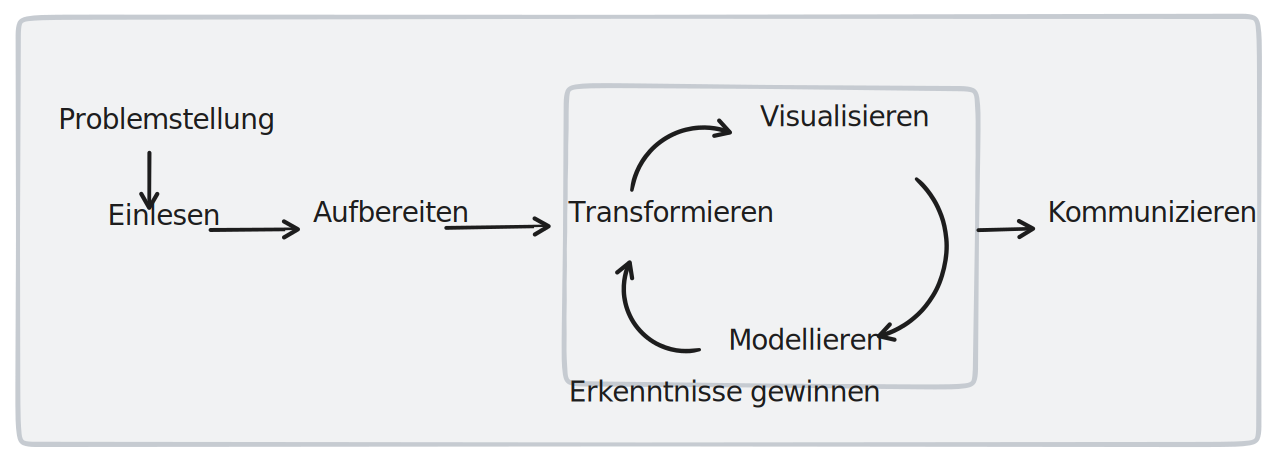
\includegraphics{Chapters/01_Chapter/../../_assets/Analyse_Prozess.svg}

}

\caption{Der Analyse-Prozess}

\end{figure}

TODO Die Abbildung verdeutlicht, dass es sich beim Analyse-Prozess um
einen iterativen und teilweise explorativen Prozess handelt. Die
Schritte ``Transformation'', ``Visualisierung'' und ``Modellierung''
sind häufig iterative Prozessschritte, bei denen man auch explorativ
vorgeht. Das bedeutet auch, man sich bewusst die Freiheit nimmt,
unterschiedliche Verfahren auszuprobieren, um neue Erkenntnisse zu
gewinnen oder dass man offen für neue Ideen und Ansätze bleibt und sich
nicht zu früh auf eine bestimmte Vorgehensweise festlegt. Durch die
iterative Durchführung dieser Schritte und das explorative Vorgehen kann
man neue Erkenntnisse gewinnen und die Analyse vertiefen.

Zudem zeigt sich, dass die Schritte ``Transformation'',
``Visualisierung'' und ``Modellierung'' im Datenanalyse-Prozess nicht
unabhängig voneinander betrachtet werden können, sondern dass sie sich
gegenseitig beeinflussen und bedingen. Beispielsweise könnte es bei der
Transformation der Daten notwendig sein, mehrere Veränderungen an den
Daten vorzunehmen, um sie für die geplante Analyse geeignet zu machen.
Durch die Visualisierung der Daten kann es jedoch möglich sein, neue
Muster oder Zusammenhänge zu erkennen, die dazu führen, dass die Daten
anders transformiert werden müssen. Ähnlich verhält es sich bei der
Modellierung der Daten. Hier können verschiedene Modelle verglichen und
iterativ verbessert werden, um die besten Vorhersagen zu erhalten. Durch
die Visualisierung der Ergebnisse kann es jedoch möglich sein, dass neue
Erkenntnisse gewonnen werden, die dazu führen, dass das Modell anders
aufgebaut werden muss. Es ist daher wichtig, dass diese Schritte nicht
unabhängig voneinander betrachtet werden, sondern dass man sich bewusst
die Freiheit nimmt, explorativ vorzugehen und die Schritte iterativ
durchzuführen, um zu sinnvollen Ergebnissen zu gelangen.

\bookmarksetup{startatroot}

\hypertarget{summary}{%
\chapter{Summary}\label{summary}}

In summary, this book has no content whatsoever.

\bookmarksetup{startatroot}

\hypertarget{references}{%
\chapter*{References}\label{references}}
\addcontentsline{toc}{chapter}{References}

\markboth{References}{References}

\hypertarget{refs}{}
\begin{CSLReferences}{1}{0}
\leavevmode\vadjust pre{\hypertarget{ref-almazmomi_impact_2021}{}}%
Almazmomi, Najah, Aboobucker Ilmudeen, und Alaa A. Qaffas. 2021. {„The
impact of business analytics capability on data-driven culture and
exploration: achieving a competitive advantage``}. \emph{Benchmarking:
An International Journal} 29 (4): 1264--83.
\url{https://doi.org/10.1108/BIJ-01-2021-0021}.

\leavevmode\vadjust pre{\hypertarget{ref-gluchowski_business_2016}{}}%
Gluchowski, Peter. 2016. {„Business {Analytics} -- {Grundlagen},
{Methoden} und {Einsatzpotenziale}``}. \emph{HMD Praxis der
Wirtschaftsinformatik} 53 (3): 273--86.
\url{https://doi.org/10.1365/s40702-015-0206-5}.

\leavevmode\vadjust pre{\hypertarget{ref-knuth84}{}}%
Knuth, Donald E. 1984. {„Literate Programming``}. \emph{Comput. J.} 27
(2): 97--111. \url{https://doi.org/10.1093/comjnl/27.2.97}.

\leavevmode\vadjust pre{\hypertarget{ref-popovic_impact_2018}{}}%
Popovič, Aleš, Ray Hackney, Rana Tassabehji, und Mauro Castelli. 2018.
{„The impact of big data analytics on firms' high value business
performance``}. \emph{Information Systems Frontiers} 20 (2): 209--22.
\url{https://doi.org/10.1007/s10796-016-9720-4}.

\leavevmode\vadjust pre{\hypertarget{ref-seiter_business_2019}{}}%
Seiter, Mischa. 2019. \emph{Business {Analytics}: {Wie} {Sie} {Daten}
für die {Steuerung} von {Unternehmen} nutzen}. 2., komplett
überarbeitete und erweiterte. München: Vahlen.

\leavevmode\vadjust pre{\hypertarget{ref-shanks_impact_2010}{}}%
Shanks, Graeme, Rajeev Sharma, Peter Seddon, und Peter Reynolds. 2010.
{„The {Impact} of {Strategy} and {Maturity} on {Business} {Analytics}
and {Firm} {Performance}: {A} {Review} and {Research} {Agenda}``}.
\emph{ACIS 2010 Proceedings}, Januar.
\url{https://aisel.aisnet.org/acis2010/51}.

\leavevmode\vadjust pre{\hypertarget{ref-wickham_r_2016}{}}%
Wickham, Hadley, und Garrett Grolemund. 2016. \emph{R for {Data}
{Science}: {Import}, {Tidy}, {Transform}, {Visualize}, and {Model}
{Data}}. "O'Reilly Media, Inc.".

\end{CSLReferences}



\end{document}
